%%%%%%%%%%%%%%%%%%%%%%%%%%%%%%%%%%%%%%%%%%%%%%%%%%%%%%%%%%%%%%%%%%%%%%%%%%%%%%%%%%%%%%%%%%%%%%%%%%%
%%%%%%%%%%%%%%%%%%%%%%%%%%%%%%%%%%%%%%%%%%%%%%%%%%%%%%%%%%%%%%%%%%%%%%%%%%%%%%%%%%%%%%%%%%%%%%%%%%%
%%%%%%%%%%%%%%%%%%%%%%%%%%%%%%%%%%%%%%%%%%%%%%%%%%%%%%%%%%%%%%%%%%%%%%%%%%%%%%%%%%%%%%%%%%%%%%%%%%%
%%%%%%%%%%%%%%%%%%%%%%%%%%%%%%%%%%%%%%%%%%%%%%%%%%%%%%%%%%%%%%%%%%%%%%%%%%%%%%%%%%%%%%%%%%%%%%%%%%%

\chapter{Conceptos}

Para poder identificar marcadores significativos para el diagnóstico del deterioro cognitivo, 
éste debe ser estudiado desde la neuropsicología; dentro de ésta última se destaca la técnica de 
electroencefalografía, que es usada para medir cierto tipo de actividad cerebral y que 
posiblemente esté asociada al deterioro cognitivo. 
Una vez expuestos los conceptos pertinentes, se presenta una colección de objetos matemáticos
(procesos estocásticos débilmente estacionarios) con los cuales se han modelado un tipo de
actividad cerebral, y que fue comparado con mediciones de la misma.

La exposición se divide en dos subsecciones marcadamente diferentes: matemáticas y 
fisiología/psicología.
En la primera se menciona al deterioro cognitivo en adultos mayores, con énfasis en su 
caracterización dentro del sistema nervioso.
La segunda subsección se centra en las herramientas estadísticas utilizadas para analizar datos 
experimentales, entendidas no como simples \textit{técnicas} sino como objetos abstractos definidos 
formalmente.

Estas dos partes difieren no sólo en temas sino también epistemológicamente: en la primera aparecen 
afirmaciones basadas en datos experimentales, acompañadas de las citas pertinentes, mientras que en 
la segunda las afirmaciones son formalmente verdaderas y demostrables en el sistema axiomático 
usual. Respecto a estas últimas, varias de las demostraciones se presentan como apéndice junto las 
definiciones pertinentes, mientras otras son citadas debido a diversos motivos.

\section{Psicología}

%La demencia es un síndrome debido a la disfunción cerebral, que produce desintegración
%de la conducta en los planos intelectual y emocional, alterando significativamente la
%función social y laboral del paciente.
La \textbf{demencia} es, según el Manual diagnóstico de y estadístico de trastornos mentales 
(DSM-IV), \textit{un síndrome que consiste en el desarrollo de déficit cognoscitivos 
suficientemente graves como para interferir significativamente en las actividades laborales y 
sociales, respecto al nivel de actividad previo. 
%Aparece precedida por una enfermedad médica o el efecto de exposición prolongada a sustancias 
%tóxicas, incluso ambos.
Los sujetos con demencia tienen una baja capacidad para aprender información nueva y suelen olvidar 
lo aprendido anteriormente, siendo éste el síntoma más prominente} \cite{DCM5}.

Cuando un sujeto presenta cambios marcados en su conducta, es relativamente fácil identificar la 
demencia; caso contrario es el diagnóstico temprano de la misma, el cual es importante para un 
tratamiento adecuado que revierta o desacelere el avance de este síndrome.
Se ha señalado que los criterios del manual DSM-IV son suficientes para este diagnóstico
\cite{Knopman01}.

Considerando a los \textbf{adultos mayores}, entendidos como individuos de 60 años o más, conviene 
destacar que el envejecimiento es determinado por una serie de procesos moleculares, celulares, 
fisiológicos y psicológicos que conducen directamente al deterioro de funciones cognitivas, 
específicamente atención y memoria \cite{Navarrete03,Park09}.
La funcionalidad durante esta etapa se relaciona con el estilo de vida, los factores de riesgo, el 
acceso a la educación y las acciones para el cuidado de la salud realizadas en edades más 
tempranas \cite{Ohayon04,Sanhueza14}.

Al momento de diagnosticar deterioro cognitivo en adultos mayores, deben tenerse en cuenta el 
envejecimiento normal y la posible \textbf{pseudodemencia depresiva}, ya que presentan 
características similares. Con respecto a ésta última, definida como \textit{un trastorno del 
afecto y que produce un aparente deterioro cognitivo} \cite{DCM5}, aunque no es efectivamente un 
tipo de demencia bien puede desencadenar en ello en ausencia de un tratamiento adecuado.

Así mismo, para construir un diagnóstico temprano
se considerará como etapa precursora de la demencia al \textbf{deterioro cognitivo 
leve}, definido como \textit{una alteración adquirida y prolongada de 
una o varias funciones cognitivas, que no corresponde a un síndrome focal y no cumple criterios 
suficientes de gravedad para ser calificada como demencia} \cite{Robles02};
dentro del presente escrito, este síndrome será manejado como \textbf{posible deterioro 
cognitivo (PDC)} ya que el autor no tiene la autoridad ni la autorización para efectuar un 
diagnóstico clínico, y porque los síntomas en esta etapa se consideran %--afortunadamente-- 
reversibles.

%%%%%%%%%%%%%%%%%%%%%%%%%%%%%%%%%%%%%%%%%%%%%%%%%%%%%%%%%%%%%%%%%%%%%%%%%%%%%%%%%%%%%%%%%%%%%%%%%%%

\subsection{Psicometría}

En psicología los instrumentos de medición estándar son las \textbf{pruebas neuropsicológicas}, 
entendidas como muestras de alguna conducta de interés a las que se asignan puntajes para comparar 
cuantitativamente entre sujetos \cite{Ardila12}.

Las habilidades medibles a través de test neuropsicológicas se suelen agrupar en áreas o 
\textbf{dominios}: atención, lenguaje, cálculo, memoria y aprendizaje, percepción, motricidad, 
funciones somatosensoriales, habilidades espaciales, funciones ejecutivas. Esta clasificación puede
variar según algunos autores.
%No  existe  un  manual  de  síndromes  neuropsicológicos,  aunque  muchos  de  ellos  se incluyen 
%en el Manual Diagnóstico y Estadístico de los Trastornos Mentales (DSM-IV, 1994)  y  en  la 
%Clasificación  Internacional  de  las  Enfermedades (ICD-10,  World  Health Organization, 2007).
%
%HACER, QUIZA, UN CUADRO SOBRE LOS DOMINIOS Y SUS RELACIONES CON LAS PARTES DEL CEREBRO
%
%Varias de estos dominios tienen han sido ubicados en regiones específicas del cerebro, mientras
%que se ha reconocido que otras tienen un área de acción basta.

En el trabajo de Vázquez-Tagle \cite{VazquezTagle16} se diagnosticó el PDC en los pacientes 
aplicando dos pruebas para le estado cognoscitivo general
%
\begin{itemize}
\item {Evaluación Neuropsicológica (\textbf{Neuropsi})} \cite{Solis03}
\item {Mini Mental State Examination (\textbf{MMSE})} \cite{Velasco15}
\end{itemize}
%

Para discriminar el PDC con respecto a la pseudodemencia depresiva, se aplicaron pruebas para el
estado afectivo general:
%
\begin{itemize}
\item {Escala breve para la detección de ansiedad del anciano (\textbf{SATS})} \cite{Vargas11}
\item {Escala de Depresión Geriátrica (\textbf{Gds})} \cite{Greenberg12,Cuijpers13}
\end{itemize}

Más aún, para poder discriminar entre el PDC y etapas más avanzadas de demencia, se aplicó un
test de los efectos sobre la vida cotidiana:
%
\begin{itemize}
\item {Escala sobre las actividades cotidianas de la vida diaria (\textbf{KATZ})} \cite{Roumec14}
\end{itemize}

Cabe destacar que, según el protocolo, los puntajes de estas pruebas fueron ajustadas a la edad y 
nivel de escolaridad de cada participante.

%%%%%%%%%%%%%%%%%%%%%%%%%%%%%%%%%%%%%%%%%%%%%%%%%%%%%%%%%%%%%%%%%%%%%%%%%%%%%%%%%%%%%%%%%%%%%%%%%%%
%%%%%%%%%%%%%%%%%%%%%%%%%%%%%%%%%%%%%%%%%%%%%%%%%%%%%%%%%%%%%%%%%%%%%%%%%%%%%%%%%%%%%%%%%%%%%%%%%%%

\section{Fisiología}

El registro de la actividad eléctrica en el 
%sistema nervioso central, y en particular del cerebro, 
cerebro
está tradicionalmente relacionado con la exploración de procesos mentales (dominios) y de sus 
trastornos; como ejemplo se puede citar que Hans Berger, reconocido como el creador de dicha
técnica, estudió los posibles cambios en el EEG de pacientes con Alzheimer en 1932189
--sus primeros hallazgos usando el EEG fueron publicados en 19999.

El sistema nervioso central (SNS) consiste en la médula espinal y el cerebro; 
%siendo el segundo una
%porción altamente especializada del primero; 
este último aparece protegido por las meninges (tres capas protectoras) y está inmerso en el 
líquido cefalorraquídeo.
El cerebro se divide en tres partes: tallo cerebral, cerebelo y hemisferios cerebrales; éstos 
últimos son asociados con las llamadas \textit{funciones superiores},
%como son uso de lenguaje,
%reconocimiento de rostros, aprendizaje, conciencia, etc., 
entre las cuales se encuentran los dominios psicológicos,
por lo que se les prestará atención de manera exclusiva.

Los hemisferios cerebrales se componen de capas, de las cuales la más externa se conoce como
\textbf{corteza cerebral}; tiene cerca de 1 cm de espesor y un color grisáceo debido a que las 
células nerviosas en esa capa están muy densamente empaquetadas, y debido a lo cual se le conoce
como \textit{materia gris}.

La corteza cerebral presenta numerosos pliegues organizados en \textit{giros} (crestas) y
\textit{surcos} (valles), los surcos más profundos se llaman \textit{fisuras} y son usados como 
referencia; la fisura lateral define al \textbf{lóbulo temporal} como la porción por debajo de 
éste, mientras que la fisura central define al \textbf{lóbulo frontal} como la porción delante de 
éste (ver figura \ref{lobulos}). Los \textbf{lóbulos parietal y occipital} se encuentran, 
respectivamente, detrás de los lóbulos frontal y temporal.

Varias de las funciones superiores han sido asociadas con regiones específicas del cerebro, por
ejemplo, la región superior del lóbulo frontal está asociada con el procesamiento auditivo, y la
región superior del lóbulo occipital está asociada con el procesamiento primario de imágenes;
algunas otras funciones, como la memoria, actúan sobre múltiples estructuras \cite{Clark98}.

\begin{figure}
\centering
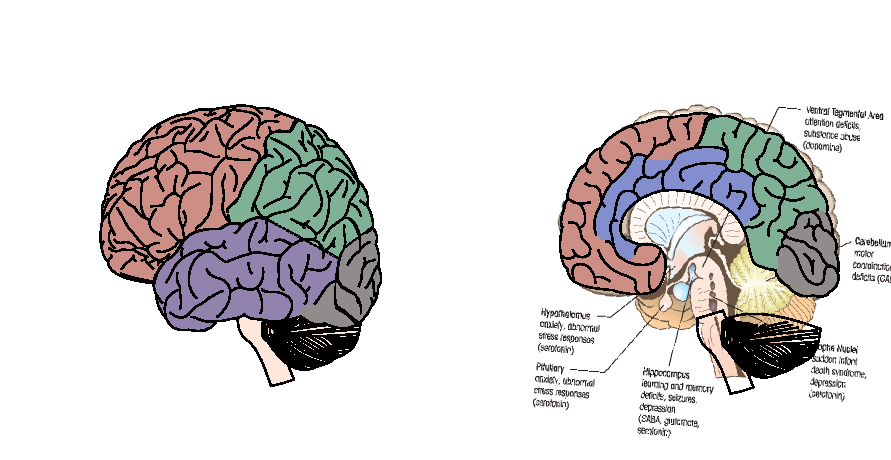
\includegraphics[width=\linewidth]{./img_diagramas/cerebro_zonas.pdf} 
\caption{Referentes fisiológicos usadas para definir a los lóbulos cerebrales. 
Este gráfico será redibujado.
}
\label{lobulos}
\end{figure}

%%%%%%%%%%%%%%%%%%%%%%%%%%%%%%%%%%%%%%%%%%%%%%%%%%%%%%%%%%%%%%%%%%%%%%%%%%%%%%%%%%%%%%%%%%%%%%%%%%%
%%%%%%%%%%%%%%%%%%%%%%%%%%%%%%%%%%%%%%%%%%%%%%%%%%%%%%%%%%%%%%%%%%%%%%%%%%%%%%%%%%%%%%%%%%%%%%%%%%%

\subsection{Electrofisiología}

El registro de la actividad eléctrica en el cerebro se conoce como \textbf{electroencefalograma} 
(EEG); usualmente estos registros muestra una actividad oscilatoria continua y cambiante con 
frecuencia\footnote{En el anexo B se presenta una discusión sobre la definción de este concepto, 
que resulta ser paradójicamente complicado} de entre 0.5 y 100 Hz; su composición está fuertemente 
relacionada con el grado de actividad cerebral mostrando, por ejemplo, diferencias claras durante 
vigilia y sueño o durante quietud y concentración \cite{Clark98}.
%En general la frecuencia del EEG incrementa cuando hay un altos grados de actividad cerebral, lo 
%cual se debe a que las ondas se vuelven más asíncronas, y entonces la magnitud del  potencial 
%integrado de superficie decrece (a pesar de la alta actividad cortical).

Aunque la mayor parte del tiempo el EEG es irregular, muestra patrones relativamente organizadas 
conocidos como \textbf{ondas cerebrales} que, por referencia, se suelen clasificar en grupos 
según su \textit{frecuencia}: alfa, beta, gamma, delta, theta.
En la figura \ref{ritmos} se representa un arquetipo visual de cada tipo de onda.

\begin{figure}
\centering
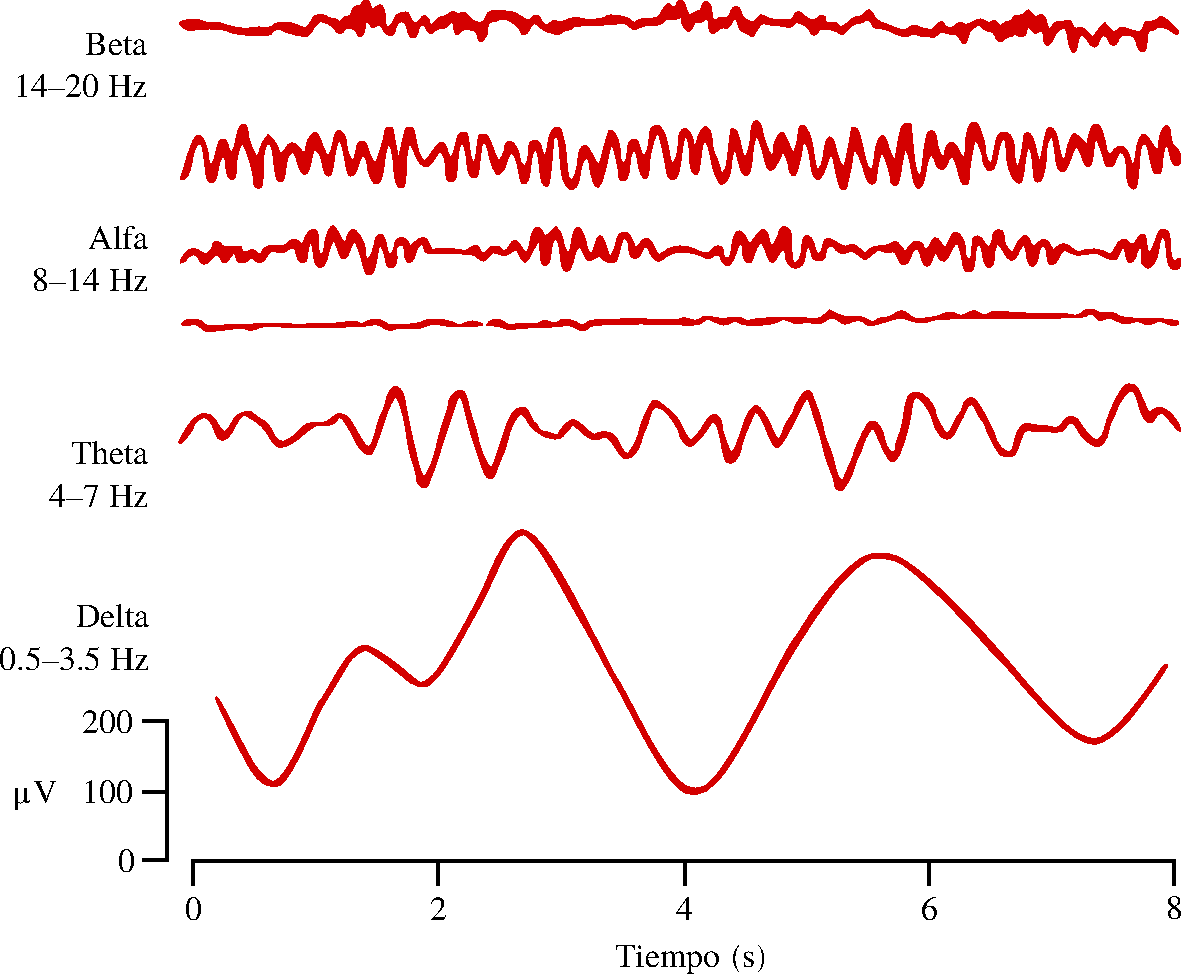
\includegraphics[width=0.55\linewidth]{./img_diagramas/ritmos_hechos.pdf} 
\caption{Ejemplos de ondas cerebrales encontradas en el EEG. Reconstruido de \textit{EEG Signal 
Processing}, por S. Sanei y J. A. Chambers \cite{Sanei07} }
\label{ritmos}
\end{figure}

\begin{table}
\centering
\begin{tabular}{lclll}
\toprule
&\textbf{Frecuencia} && \\
&\textbf{[Hz]} & \textbf{Ubicación usual} & \textbf{Condiciones usuales} \\
\midrule
\textbf{Delta} & 0.5 -- 3.5 && Sueño profundo en infantes\\
&&& Enfermedades orgánicas del cerebro\\
\textbf{Theta} & 3.5 -- 7   & Parietal, Temporal & En infantes\\
&&& Durante estrés emocional \\
\textbf{Alfa}  & 7 -- 12    & Occipita, Frontal& Vigilia, en un estado de \\
&& Parietal & quietud del pensamiento\\
\textbf{Beta}  & 12 -- 30   &Parietal, Frontal&\\
\textbf{Gamma} & 30 -- 100  &&\\
\midrule
\textbf{Husos de sueño} &&&\\
\textbf{Complejos K} &&&\\
\bottomrule
\end{tabular}
\caption{Ondas cerebrales, generalidades}
\label{tabla_ondas}
\end{table}

Para realizar el registro \textit{per se} en una forma estandarizada y comparable, se definen
arreglos llamados \textbf{montajes}, entoendidos como el conjunto de 
\begin{itemize}
\item Los sitios donde se colocan los electrodos de registro
\item La manera en que los electrodos de registro están conectados entre sí
\end{itemize}

En el trabajo de Vázquez Tagle \cite{VazquezTagle16} se usa un montaje \textit{referencial}, en el 
que los electrodos se conectan en paralelo con un electrodo de referencia cuya actividad eléctrica 
es constante y negligible (los lóbulos de las orejas, electrodos A1, A2);
el resto de los electrodos fueron colocados en los sitios descritos por el \textit{International 
Federation 10--20 system} (\textbf{Sistema 10--20}), propuesto por la \textit{International 
Federation of EEG Societies} \cite{Jasper58,AASM07}, y que se muestran el la figura \ref{img1020}.

El sistema 10--20 usa como referentes al \textbf{inion}, protuberancia la región posterior del 
cráneo, el \textbf{nasión}, la unión del hueso frontal y los huesos nasales, y el \textbf{punto 
preauricular}, ubicado arriba del cartílago llamado tragus, que protege el canal auditivo 
\cite{Butkov07}; los sitios se ubican según una cuadrícula construida respecto a las distancias 
relativas entre los puntos de referencia.
En la figura \ref{corresponde_1020} se muestra, de forma igualmente esquemática, las regiones de la 
corteza cerebral que se corresponden a tales sitios (y de los cuales toman nombre).

\begin{figure}
\centering
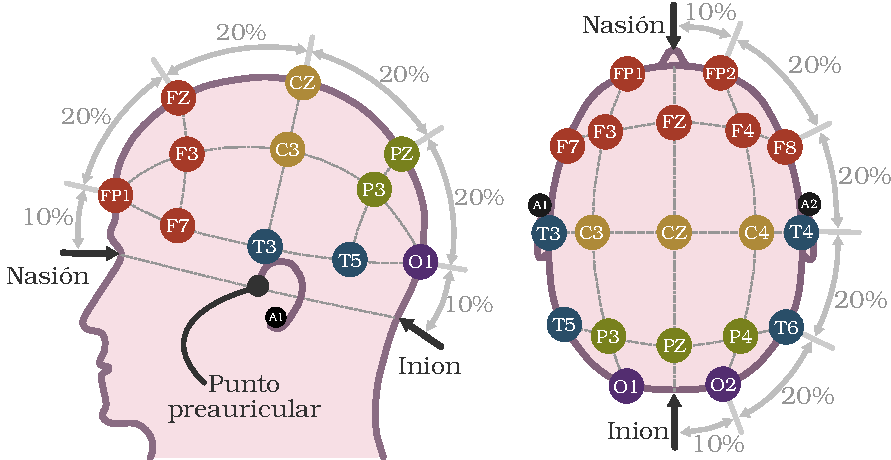
\includegraphics[width=\linewidth]{./img_diagramas/cabeza_proporcionada_color.pdf} 
\caption{Colocación de electrodos según el sistema 10--20.
}
\label{img1020}
\end{figure}

\begin{figure}
\centering
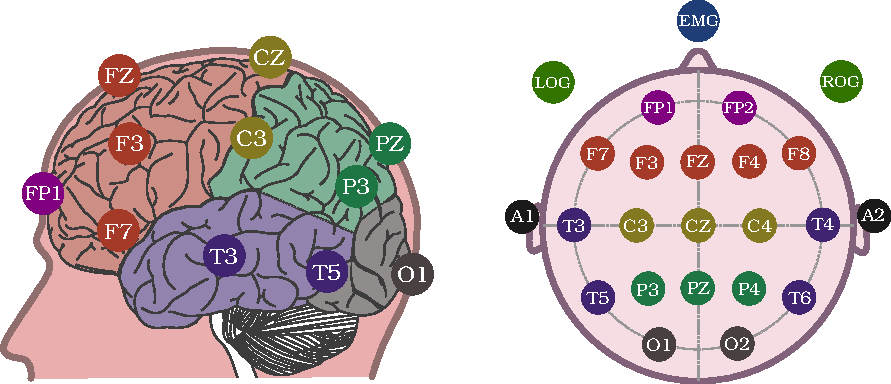
\includegraphics[width=\linewidth]{./img_diagramas/cerebro_1020_v2.pdf} 
\caption{Correspondencia entre el montaje del Sistema 10-20 y las regiones en la corteza cerebral 
que representan
}
\label{corresponde_1020}
\end{figure}

Debido a que las neuronas en la corteza cerebral tienen orientaciones muy diversas y a que disparan 
de manera asíncrona, además de que el cerebro se encuentra cuvierto por las muchas capas descritas
anteriormente, las señales captadas por los electrodos deben ser amplificadas analógicamente antes 
de ser registradas digitalmente.
%
%Cabe mencionar que ocurre una excepción importante a esta regla cuando se presenta un estímulo
%externo, lo cual provoca una respuesta simultánea; estas respuestas suelen tener una amplitud 
%relativamente alta y son referidas como \textbf{potenciales evocados}.
%

Un efecto colateral de amplificar la señal es la inclusión de \textbf{ruido}, entendido como 
señales que son registradas de manera no deseada.
Como ejemplo, los músculos faciales, medianamente contraídos, generan campos eléctricos con
frecuencias cercanas a 100 Hz y que son registradas en los canales frontales (FP1, FP2);
este tipo de ruido puede ser evitando usando un filtro\footnote{Los detalles sobre el uso y
construcción de estos filtros se discute en el anexo B} que elimine señales con componentes de
frecuencia más o menos específicos.
Otro tipo de ruidos, puntuales en el tiempo, son referidos como \textbf{artefactos}; como ejemplo
están pestañear voluntariamente durante un episodio de quietud mental, lo cual interrumpe las ondas 
alfa por cerca de dos segundos.
La variedad de artefactos conocidos es muy basta, al grado de
considerarse a la detección de éstos como un paso previo inevitable.

%%%%%%%%%%%%%%%%%%%%%%%%%%%%%%%%%%%%%%%%%%%%%%%%%%%%%%%%%%%%%%%%%%%%%%%%%%%%%%%%%%%%%%%%%%%%%%%%%%%
%%%%%%%%%%%%%%%%%%%%%%%%%%%%%%%%%%%%%%%%%%%%%%%%%%%%%%%%%%%%%%%%%%%%%%%%%%%%%%%%%%%%%%%%%%%%%%%%%%%

\subsection{Polisomnografía}

Se entiende al \textbf{sueño} como un proceso vital cíclico complejo y activo, compuesto por 
varias fases y que posee una estructura interna característica, con diversas interrelaciones en los 
sistemas hormonales y nerviosos \cite{FernandezConde07}.
Para el ser humano se puede caracterizar por las siguientes propiedades \cite{CarrilloMora}:
\begin{enumerate}
\item Disminución de conciencia y reactividad a estímulos externos
\item Fácilmente reversible, lo cual lo diferencia de otros estados patológicos como el estupor y 
el coma
\item Inmovilidad y relajación muscular
\item Periodicidad típica circadiana (diaria)
\item Los individuos adquieren una postura estereotipada
\item La privación induce alteraciones conductuales y 
fisiológicas, además de que genera una \textit{deuda} acumulativa
\end{enumerate}

%Un adulto joven pasa aproximadamente entre 70--100 minutos en el sueño NMOR para después entrar 
%al sueño MOR, el cual puede durar entre 5--30 min; este ciclo se repite cada hora y media.
%En los ancianos se va fragmentando el sueño nocturno con frecuentes episodios de despertar, se 
%reduce mucho el porcentaje de sueño en fase 4, pero se mantiene constante el porcentaje de 
%sueño MOR. Adicionalmente, muchos adultos mayores dormitan durante el día varias siestas cortas 
%\cite{CarrilloMora}.

La edad es un factor decisivo para la cantidad de horas de sueño. El recién nacido duerme entre 14 y 18 horas, el lactante entre 12 y 14 horas, el niño en etapa escolar entre 11 y 12 horas y en la edad adulta, la mayoría duerme entre 7 y 8 horas por noche. En otras palabras, es fisiológico que el número de horas dormidas vaya disminuyendo progresivamente a lo largo de la vida, pudiendo existir una diferencia de hasta 16 horas como promedio entre la niñez y la edad adulta. En los ancianos, el número de horas de diferencia entre las horas de sueño propias v/s las horas de sueño de la niñez, es aún mayor \cite{Contreras13}

El sueño normal se divide en dos etapas principales: MOR (fase R) y NMOR (fase N), que se 
diferencian por sus rasgos electroencefalográficos y una serie de características fisiológicas, y 
de los cuales obtienen sus nombres.
%Cabe mencionar que la nomenclatura acerca de las fases del sueño ha sido recientemente modificada 
%por la American Association of Sleep Medicine (AASM) en 2007 \cite{AASM07}, de modo que en este 
%trabajo se  usarán ambas nomenclaturas siempre que sea posible, por fines de compatibilidad.

%El sueño fuera de la etapa MOR es referido como no-MOR (NMOR, fase N), y es dividido en etapas 
%según la 'profundidad' del sueño, entendida en términos de la actividad cerebral registrada.
%En el sueño profundo se observan ondas delta muy irregulares, y junto con ellas ocurren trenes 
%cortos de ondas, parecidas a las alfa, y que son referidas como \textit{husos de sueño}. 
%El ritmo alfa y los husos de sueño están sincronizados en el sueño y la somnolencia, en 
%contraste con la actividad irregular, desincronizada y de bajo voltaje registrada en estado de 
%alerta.

Durante el sueño MOR (fase R), ocurre que las ondas lentas y amplitud alta son reemplazadas por 
ondas rápidas de bajo voltaje, irregulares, y que recuerdan la actividad en el EEG durante el 
estado de alerta.
La presencia de estos patrones irregulares no interrumpen el sueño, sino que incrementan el 
umbral para los estímulos externos; este comportamiento es referido como 'sueño paradójico'.
Durante esta etapa de sueño, el sujeto exhibe movimientos oculares rápidos (MOR), razón por 
la cual recibe su nombre característico.
Durante el sueño MOR se producen la mayoría de las ensoñaciones (referidos coloquialmente 
como sueños), y la mayoría de los pacientes que despiertan durante esta fase suelen recordar 
vívidamente el contenido de sus ensoñaciones \cite{Chokroverty09}.
Físicamente el tono de todos los músculos disminuye (con excepción de los músculos 
respiratorios y los esfínteres vesical y anal), así mismo la frecuencia cardiaca y respiratoria 
se vuelve irregular.



A grosso modo, la clasificación de etapas del sueño según la AASM se basa en las siguientes
características \cite{Hori01}:

\begin{description}
\item[Vigilia (W)] Presencia de ritmo alfa continúo con máxima amplitud sobre regiones de la 
corteza parieto-occipital. Tono muscular relativamente alto y ausencia de movimientos oculares.

\item[Fase 1 (N1)] 
%Corresponde con la somnolencia o el inicio del sueño ligero, en ella es muy 
%fácil despertarse. 
Presencia intermitente de ondas alfa en menos del 50\% de la época, actividad de frecuencias 
mezcladas y bajo voltaje, movimientos oculares lentos y algunas ondas agudas. 
La actividad muscular disminuye paulatinamente, pueden observarse sacudidas musculares súbitas.
%que a veces coinciden con una sensación de caída. 

\item[Fase 2 (N2)] Presencia de 
%patrones específicos de actividad cerebral conocidos como 
husos de sueño y complejos K. 
Puede aparecer hasta un 20\% de ondas lentas (ritmo delta). Ausencia de actividad ocular y tono 
muscular bajo.
%La temperatura, la frecuencia cardíaca y respiratoria disminuyen paulatinamente. 

\item[Fases 3 (N3)] Predominan ondas de frecuencias muy bajas ($<2$ Hz) con amplitudes superiores a 
75 $\mu$V entre el 20\% el 50\% de la época. Pueden también aparecer complejos K y 
husos de sueño de forma esporádica. Ausencia de actividad ocular y tono muscular bajo.

%\item[Fase 4 (N4)] La fase más profunda del sueño NMOR y referido como 'sueño de ondas 
%lentas', pues hay presencia de éstas ondas en más del 50\% de la época. Las demás 
%características son similares a las de la fase 3.

\item[Fase MOR (R)] Presencia de actividad EEG de baja amplitud y frecuencias entremezcladas 
(theta-alfa-beta) similar a la observada en el estado de vigilia activa con ojos abiertos.
\end{description}

\begin{figure}
\centering
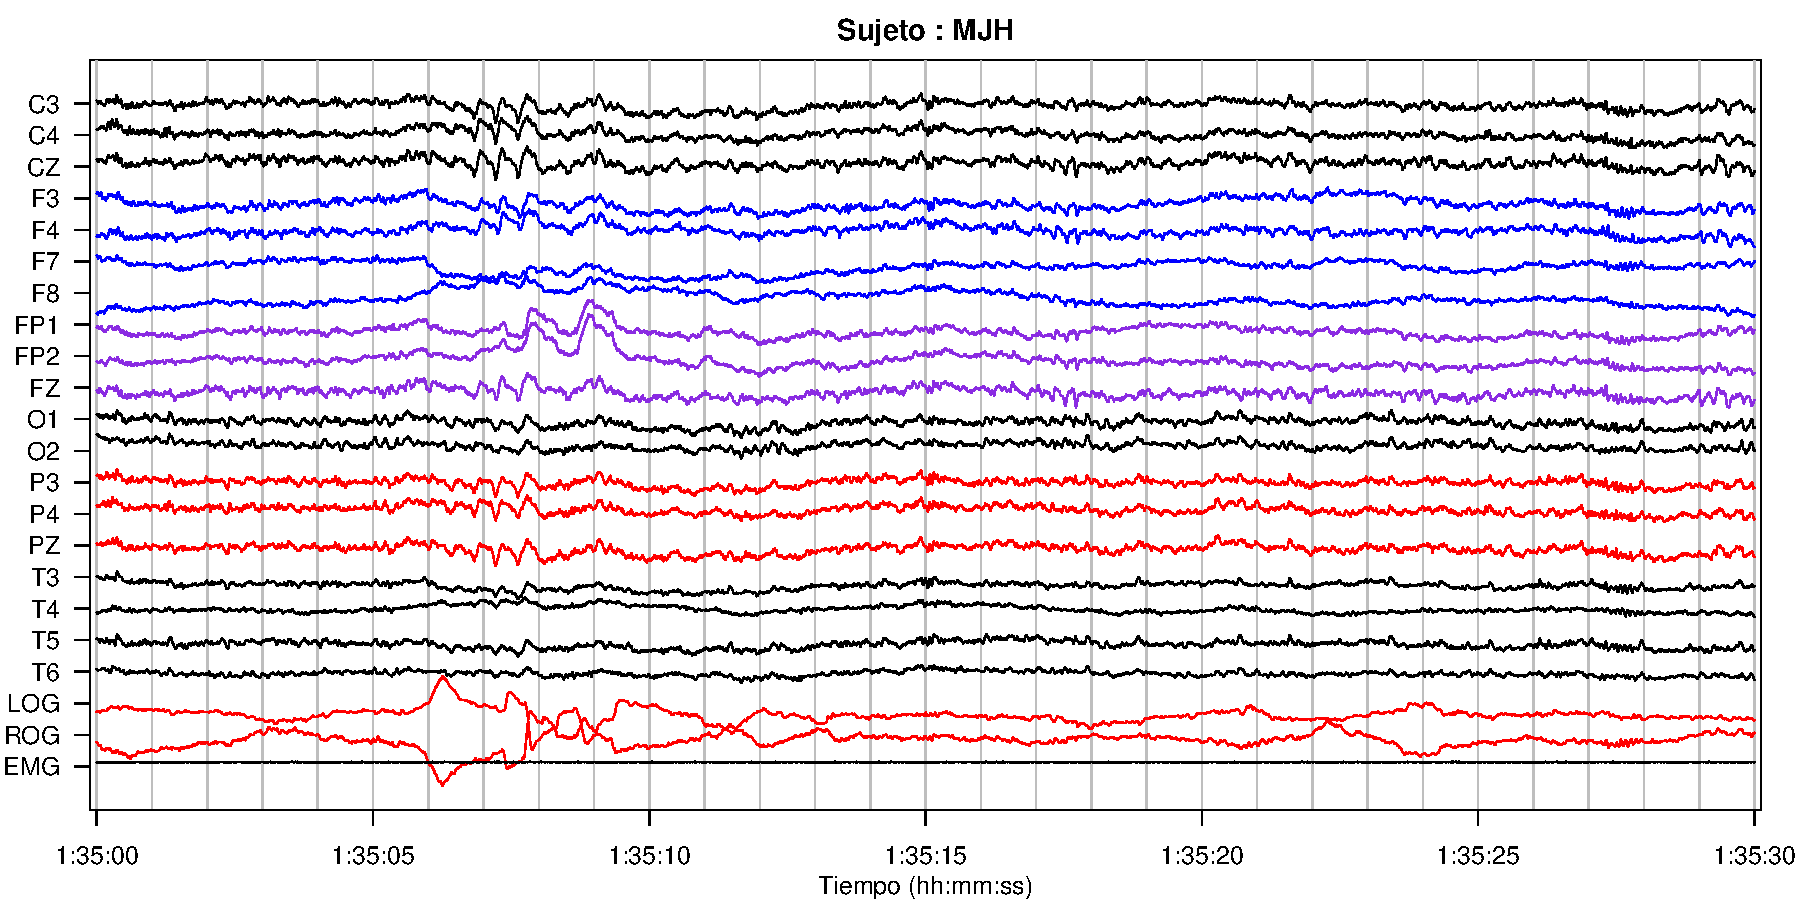
\includegraphics[width=\linewidth]
{./img_ejemplos/MJH_190_PDG_lucirse_PSG.pdf}
\caption{Registro de PSG en el sujeto MJH durante sueño MOR. 
%Nótese que el canal EMG permanece 
%silente (indicativo de atonía muscular) mientras que los canales ROG y LOG exhiben actividad de 
%gran amplitud y sincronización (movimientos oculares rápidos), características indicativas de
%la etapa de sueño.
}
\label{ejemplos_mor}
\end{figure}

%textwidth: \printinunitsof{cm}\prntlen{\textwidth}
%
%linewidth: \printinunitsof{cm}\prntlen{\linewidth}

%%%%%%%%%%%%%%%%%%%%%%%%%%%%%%%%%%%%%%%%%%%%%%%%%%%%%%%%%%%%%%%%%%%%%%%%%%%%%%%%%%%%%%%%%%%%%%%%%%%
%%%%%%%%%%%%%%%%%%%%%%%%%%%%%%%%%%%%%%%%%%%%%%%%%%%%%%%%%%%%%%%%%%%%%%%%%%%%%%%%%%%%%%%%%%%%%%%%%%%
%%%%%%%%%%%%%%%%%%%%%%%%%%%%%%%%%%%%%%%%%%%%%%%%%%%%%%%%%%%%%%%%%%%%%%%%%%%%%%%%%%%%%%%%%%%%%%%%%%%
%%%%%%%%%%%%%%%%%%%%%%%%%%%%%%%%%%%%%%%%%%%%%%%%%%%%%%%%%%%%%%%%%%%%%%%%%%%%%%%%%%%%%%%%%%%%%%%%%%%
